\documentclass{beamer}

\mode<presentation>
\setbeamerfont{footnote}{size=\tiny}
\setbeamertemplate{navigation symbols}{}

\usetheme{Warsaw}

\usepackage[backend=bibtex,style=verbose]{biblatex}
\usepackage{graphicx}

\usepackage{tikz}
\usetikzlibrary{backgrounds,positioning,fit}
\usepackage{adjustbox}

\usepackage[linesnumbered,lined,noline,ruled,noend]{algorithm2e}
\usepackage{subfig}
\usepackage{pgfplots}

\AtBeginSection[]
{
	\begin{frame}
		\frametitle{Outline}
		\tableofcontents[currentsection]
	\end{frame}
}

\bibliography{./bibs/Asynchronous-Applications,./bibs/Asynchronous-FT,./bibs/Asynchronous-Theoretical,./bibs/Example-Problems,./bibs/Fault-Tolerance,./bibs/Fixed-Point,./bibs/General-HPC,./bibs/HPC-Math-Software,./bibs/Iterative-Methods,./bibs/Preconditioning,./bibs/Self-Citations,./bibs/Textbooks}

\title[Randomized Asynchronous Linear Solvers]{Dynamic Non-Uniform Randomization in Asynchronous Linear Solvers}
\author[Coleman \& Sosonkina]{Evan Coleman and Masha Sosonkina}

\date{}

\begin{document}

%------------------------------------------------------------------------------
% Front matter
%
\begin{frame}
	\titlepage
\end{frame}


\begin{frame}
	\frametitle{Outline}
	\tableofcontents
\end{frame}

\section{Introduction}

\begin{frame}
	\frametitle{Big picture (1/3)}
	\begin{itemize}
		\item Problem: solve the linear system $Ax = b$
			\begin{itemize}
				\item $A$ is a matrix representing the system being described
				\item $x^{(k)} \in \mathbb{R}^n$ is the solution vector that will be found iteratively
				\item $b \in \mathbb{R}^n$ is some (possibly non-zero) right-hand side
			\end{itemize}
		\item Systems of linear algebraic equations arise everywhere
			\begin{itemize}
				\item Often from discretizations of partial differential equations
				\item The size of the problem can vary from $10^2 - 10^{10}$ unknowns
			\end{itemize}
		\item Solution of linear systems takes up a large portion of the available compute time on High Performance Computing (HPC) resources
		\item Creation of new and improved techniques offers chances for higher throughput or higher fidelity (or both)
	\end{itemize}	
\end{frame}
% Pictures of basic finite element problem -> matrix
%  HPC cluster

\begin{frame}
	\frametitle{Big picture (2/3)}
	\begin{itemize}
		\item For sufficiently large problems, direct solution methods are no longer viable and iterative methods are used
			\begin{itemize}
				\item Popular state-of-the art techniques include Krylov subspace solvers and multigrid methods 
			\end{itemize}
		\item The methods being discussed here are part of a class of iterative methods known as stationary linear solvers
			\begin{itemize}
				\item Examples include Jacobi and Gauss-Seidel
			\end{itemize}
		\item The more novel features involve expanding on techniques for parallelism via:
			\begin{itemize}
				\item asynchronous operation between processors
				\item randomized work selection
			\end{itemize} 
	\end{itemize}	
\end{frame}

\begin{frame}
	\frametitle{Big picture (3/3)}
	\begin{itemize}
		\item If $A$ is sufficiently ``nice'' (i.e. $\rho(A) < 1$), these new methods can be used by themselves
			\begin{itemize}
				\item Advantages:
					\begin{itemize}
						\item They scale well
						\item They solve provide a quick initial reduction in residual error
					\end{itemize}
			\end{itemize} 
		\item If $A$ is less nice, these new methods would be better to be used in conjunction with existing techniques
			\begin{itemize}
				\item As preconditioners for Krylov subspace methods
				\item As smoothers for multigrid methods
			\end{itemize}
	\end{itemize}	
\end{frame}

\section{Traditional Stationary Solvers}

\begin{frame}
	\frametitle{Solving the system}
	\begin{itemize}
		\item Assume $A$ is invertible (so the system has a unique solution)
		\item Write the $i^{th}$ equation of the system $Ax = b$ out:
			\begin{equation}
				\sum_{j=1}^n a_{ij}x_j = b_i
			\end{equation}
		\item Further assume that $a_{ii} \neq 0$, then each component can be written
			\begin{equation}
				x_i = \frac{-1}{a_{ii}}\left( \sum_{j\neq i} a_{ij}x_j - b_i \right)
			\end{equation}
		\item Performing iteration on this is known as the Jacobi algorithm
	\end{itemize}	
\end{frame}

\begin{frame}
	\frametitle{Jacobi algorithm}
	\begin{algorithm}[H]
		\DontPrintSemicolon
		\KwIn{$a_{ij} \in A$, initial guess $x^{(0)}$, RHS $b$}
		\For {$k = 1, 2, \ldots$ until convergence} {
			\For {$i = 1, 2, \ldots, n$} {
				$x_i^{(k)} = \frac{-1}{a_{ii}}\left( \sum_{j\neq i} a_{ij}x_j^{(k-1)} - b_i \right)$\;
			}
		}
	\end{algorithm}
	\begin{itemize}
		\item Convergence is guaranteed when $A$ is diagonally dominant
		\item Known as an additive method since all component updates use the prior values of $x$
			\begin{itemize}
				\item In contrast to multiplicative methods such as Gauss-Seidel that use the latest information available
			\end{itemize}
		%\item Expressing in block form: $x^{(k)} = $
	\end{itemize}
\end{frame}

\begin{frame}
	\frametitle{Gauss-Seidel algorithm}
	\begin{algorithm}[H]
		\DontPrintSemicolon
		\KwIn{$a_{ij} \in A$, initial guess $x^{(0)}$, RHS $b$}
		\For {$k = 1, 2, \ldots$ until convergence} {
			\For {$i = 1, 2, \ldots, n$} {
				$x_i^{(k)} = \frac{-1}{a_{ii}}\left( \sum_{j < i} a_{ij}x_j^{(k)} + \sum_{j > i} a_{ij}x_j^{(k-1)} - b_i \right)$\;
			}
		}
	\end{algorithm}
	\begin{itemize}
		\item Convergence tends to be better than Jacobi, but parallelism is limited
		\item For both algorithms, convergence can be judged by progression of the residual,
			\begin{equation}
				r^{(k)} = b - Ax^{(k)}
			\end{equation}
			  which will decrease to 0 as iteration proceeds
	\end{itemize}
\end{frame}

\begin{frame}
	\frametitle{Southwell algorithm}
	\begin{algorithm}[H]
		\DontPrintSemicolon
		\KwIn{$a_{ij} \in A$, initial guess $x^{(0)}$, RHS $b$}
		\For {$k = 1, 2, \ldots$ until convergence} {
			Evaluate $r^{(k)} = b - Ax^{(k)}$ \;
			Choose $i$ such that $r_i^{(k)} = b_i - Ax^{(k)}_i$ is maximized \;
			$x_i^{(k)} = \frac{-1}{a_{ii}}\left( \sum_{j\neq i} a_{ij}x_j^{(k-1)} - b_i \right)$\;
		}
	\end{algorithm}
	\begin{itemize}
		\item Convergence tends to be better still
		\item There is an added cost associated with calculating the residual so regularly (which may be done anyway to detect convergence/termination), and the algorithm is only worth using if the decrease in total number of iterations outweighs the increased cost per iteration
	\end{itemize}
\end{frame}

\begin{frame}
	\frametitle{Why do we care?}
	\begin{itemize}
		\item Classical methods are very rarely used by themselves
			\begin{itemize}
				\item Often used as preconditioners to more complex methods (e.g. Krylov subspace methods), or as smoothers in multigrid methods
			\end{itemize}
		\item Jacobi is an ``embarrassingly parallel'' problem, where parallelism can be exploited pretty fully
		\item The ideas translate directly to other similar solvers 
			\begin{itemize}
				\item i.e. many popular approaches in convex optimization
			\end{itemize}
	\end{itemize}	
\end{frame}


\section{Parallel Algorithms}

\begin{frame}
	\frametitle{Overview}
	\begin{itemize}
		\item Most problems of interest in scientific computing are very large scale in nature
		\item The number of unknowns tends to be several orders of magnitude higher than the number of processors
		\item Many different approaches to parallelism have been attempted
		\item Goals for an approach:
			\begin{itemize}
				\item Efficient (works quickly)
				\item Robust (works on a variety of problems)
				\item Scalable (works on a variety of architectures)
				\item Provable convergence and convergence rate (have meaningful bounds on how long things will take)
			\end{itemize}
	\end{itemize}	
\end{frame}

\begin{frame}
	\frametitle{Approach: block methods}
	\begin{itemize}
		\item Divide the domain into $m$ subdomains, $\mathbb{R}^n = \mathbb{R}^{n_1} \times \mathbb{R}^{n_2} \times \cdots \mathbb{R}^{n_m}$, where $n = \sum_i n_i$
		\item They don't need to be disjoint (and convergence can actually be better when they're not), but conceptually it's easier to visualize them this way
		\item Focus is on how this process can be accelerated by changing the parallel nature of the algorithm
		\item Each time a block is selected it performs one or more internal iterations of a stationary solver
	\end{itemize}
\end{frame}

\begin{frame}[shrink]
	\frametitle{Notional block picture}
	\begin{figure}[H]
		\scalebox{1.0}{
			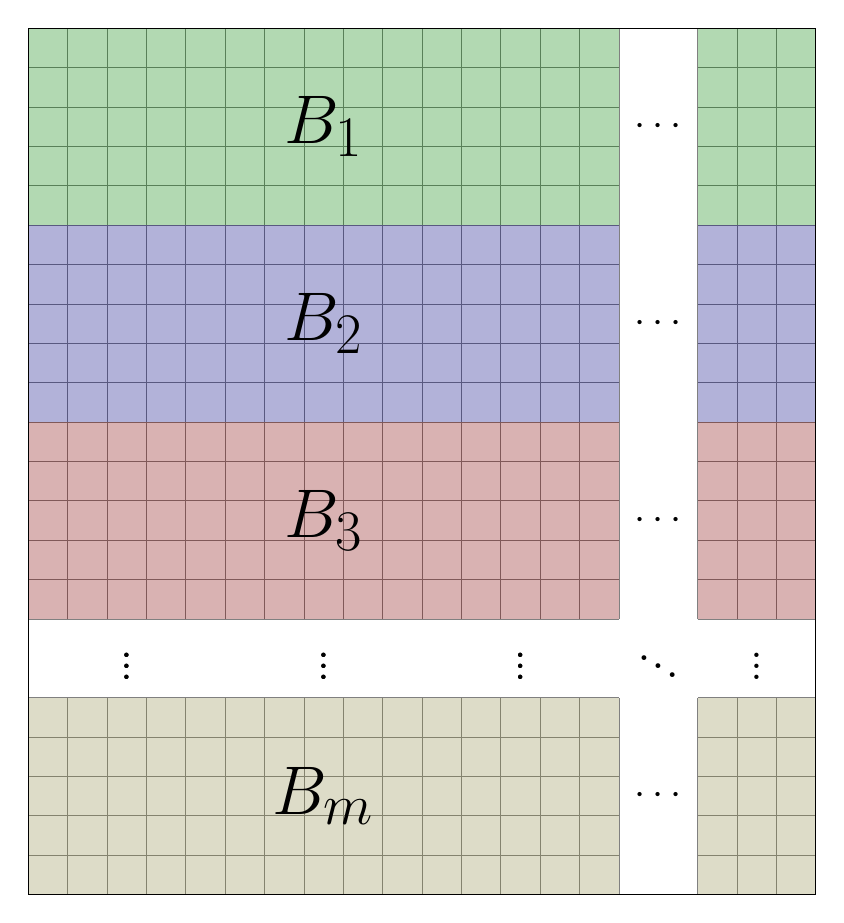
\begin{tikzpicture}
			\draw[step=5mm,gray,very thin] (0,0) grid (7.5,7.5);
			
			\draw[step=5mm,gray,very thin] (0,0) grid (7.5,7.5);
			\draw[step=5mm,gray,very thin] (0,-3.5) grid (7.5,-1);
			
			\draw[step=5mm,gray,very thin] (8.49999,-3.5) grid (10,-1);
			\draw[step=5mm,gray,very thin] (8.49999,0) grid (10,7.5);
			
			\fill[yellow!50!black,opacity=0.3]   (0,-3.5) rectangle (7.5,-1);
			\fill[yellow!50!black,opacity=0.3]   (8.49999,-3.5) rectangle (10,-1);
			
			\fill[green!50!black,opacity=0.3] (0,7.5) rectangle (7.5,5);
			\fill[green!50!black,opacity=0.3] (8.49999,7.5) rectangle (10,5);
			
			\fill[blue!50!black,opacity=0.3]  (0,5) rectangle (7.5,2.5);
			\fill[blue!50!black,opacity=0.3]  (8.49999,5) rectangle (10,2.5);
			
			\fill[red!50!black,opacity=0.3]   (0,2.5) rectangle (7.5,0);
			\fill[red!50!black,opacity=0.3]   (8.49999,2.5) rectangle (10,0);
			
			\node at (8, -2.25) {\bf \Large $\cdots$};
			\node at (8, 1.25) {\bf \Large $\cdots$};
			\node at (8, 3.75) {\bf \Large $\cdots$};
			\node at (8, 6.25) {\bf \Large $\cdots$};
			
			\node at (1.25, -0.5) {\bf $\vdots$};
			\node at (3.75, -0.5) {\bf $\vdots$};
			\node at (6.25, -0.5) {\bf $\vdots$};
			\node at (9.25, -0.5) {\bf $\vdots$};
			
			\node at (8, -0.5) {\bf \large $\ddots$};
			
			\node at (1.25, -0.5) {\bf $\vdots$};
			\node at (3.75, -0.5) {\bf $\vdots$};
			\node at (6.25, -0.5) {\bf $\vdots$};
			
			\node at (3.75, -2.25) {\Huge \bf $B_{m}$};
			\node at (3.75, 1.25) {\Huge \bf $B_3$};
			\node at (3.75, 3.75) {\Huge \bf $B_2$};
			\node at (3.75, 6.25) {\Huge \bf $B_1$};
			
			\draw[black] (0,7.5) rectangle (10,-3.5);
			\end{tikzpicture}
		}
	\end{figure}
\end{frame}

\begin{frame}
	\frametitle{Generic block algorithm}
	\begin{algorithm}[H]
		\DontPrintSemicolon
		\For {each processing element $P_{l}$} {
			\For {$i = 1, 2, \ldots$ until convergence} {
				Pick a block $j \in \{1, 2, \ldots, m\}$ {\em{\underline{somehow}}} \; 
				Read the corresponding entries of $A, x, b$ \;
				Perform Jacobi or Gauss-Seidel relaxations for all equations in block $j$ \;
				Update the data for block $j$ \;
			}
		}
	\end{algorithm}
	\begin{itemize}
		\item The way that each processor selects the block it works on can alter convergence
		\item Before going into block selection strategies, first a brief aside regarding synchronous and asynchronous updates
	\end{itemize}
\end{frame}


\begin{frame}
	\frametitle{Fixed Point Methods}
	\begin{itemize}
		\item The solvers focused on here can all be expressed as fixed point iterations of the form
			\begin{equation}
				x = G(x)
			\end{equation}
		\item In terms of parallelism for these methods:
		\begin{itemize}
			\item Each component (or block of components) can be treated as a task and assigned to a single processor
			\item Each processor {\em should} be able to complete its current task without receiving new information from other processors 
		\end{itemize}
	\end{itemize}
\end{frame}

% Synchronous
\begin{frame}[shrink]
	\frametitle{Synchronous Fixed Point Iteration}
	\begin{itemize}
		\item The fixed point iteration $x = G(x)$ can be broken into the individual component functions $g_i(x)$ that update each element $x_i$ of $x$ where $x = G(x) = (g_1(x), g_2(x), \cdots, g_n(x))$:
		\begin{align*}
		x_1^{(k+1)} &= g_1(x_1^{(k)}, x_2^{(k)}, x_3^{(k)}, \cdots, x_n^{(k)}) \\
		x_2^{(k+1)} &= g_2(x_1^{(k)}, x_2^{(k)}, x_3^{(k)}, \cdots, x_n^{(k)}) \\
		x_3^{(k+1)} &= g_3(x_1^{(k)}, x_2^{(k)}, x_3^{(k)}, \cdots, x_n^{(k)}) \\
		&\vdots							   \\
		x_n^{(k+1)} &= g_n(x_1^{(k)}, x_2^{(k)}, x_3^{(k)}, \cdots, x_n^{(k)}) 		
		\end{align*}
		\item In the synchronous case, all updates $g_i(x)$ use {\em the same} values for all components of the vector $x$
		\item Results will be reproducible since the same updates will occur in the same order every time
	\end{itemize}
\end{frame}

% Asynchronous
\begin{frame}[shrink]
	\frametitle{Asynchronous Fixed Point Iteration}
	\begin{itemize}
		\item Let $s_l(k)$ indicate the number of times that the $l^{th}$ component has been updated after the $k^{th}$ update
		\item Let $I^{(k)}$ be a set of indices that specifies which components to update at the $k^{th}$ update
		\item Then under standard fairly mild assumptions, the $(k+1)^{st}$ update to the $i^{th}$ component, $x_i$, can be written
		{\small
			\begin{equation}
			x_i^{(k+1)} = \begin{cases} 
			x_i^{(k)} \hspace{1.55in} \text{ if } i \notin I^{(k+1)} \\
			g_i(x_1^{(s_1(k))}, x_2^{(s_2(k))}, \cdots, x_n^{(s_n(k))}) \text{ if } i \in I^{(k+1)}
			\end{cases}
			\end{equation}
		}
		\item In the asynchronous case, the updates $g_i(x)$ use {\em different} values for $x_i \in x$ 
		\begin{itemize}
			\item i.e. each update will use the latest values available to it
		\end{itemize}
		\item Update order is non-deterministic and is related to the parallel performance of the hardware
	\end{itemize}
\end{frame}

\begin{frame}
	\frametitle{Synchronous Update}
	\begin{figure}
		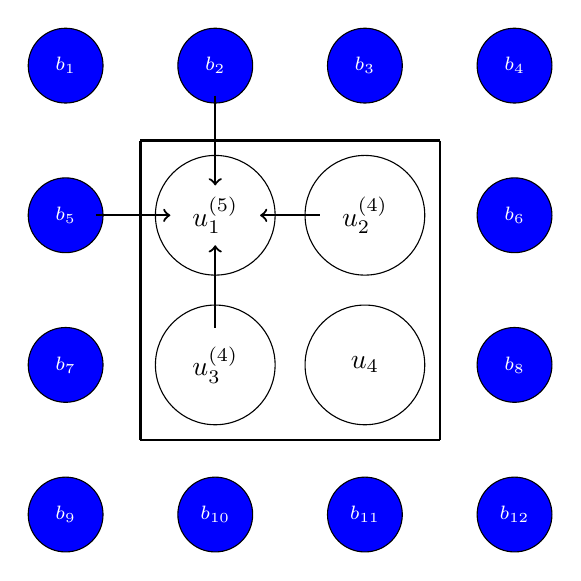
\begin{tikzpicture}[scale=1.9]
		% setup the nodes as small black circles
		\foreach \x in {0,...,3} {
			\foreach \y in {0,...,3} {
				\node[shape=circle,fill=black,scale=0.3] (\x-\y) at (\x,\y){}; 
				%labeling as \x-\y allows referencing inside of a foreach loop later
			}
		}
		
		% circle interior nodes with letters
		\foreach \mynode/\mytext in {1-2/$u_1^{(5)}$,2-2/$u_2^{(4)}$,1-1/$u_3^{(4)}$,2-1/$u_4$} {
			\draw[fill=white] (\mynode) circle (0.4cm) node {\mytext};
		}	
		
		% 
		\draw[thick] (0.5,0.5) to (2.5,0.5); 
		\draw[thick] (0.5,0.5) to (0.5,2.5); 
		\draw[thick] (0.5,2.5) to (2.5,2.5); 
		\draw[thick] (2.5,2.5) to (2.5,0.5); 
		
		% label boundary nodes
		\foreach \mynode/\mytext in {0-3/$b_1$,1-3/$b_2$,2-3/$b_3$,3-3/$b_4$,
			0-2/$b_5$,0-1/$b_7$,3-1/$b_8$,3-2/$b_6$,
			0-0/$b_9$,1-0/$b_{10}$,2-0/$b_{11}$,3-0/$b_{12}$} {
			\draw[fill=blue,text=white] (\mynode) circle (0.25cm) node {{\scriptsize \mytext}};
		}	
		
		% drawing lines to show the nodes needed to update $u_1$
		\draw[->,thick] (0.2,2) to (0.7,2); 
		\draw[->,thick] (1,2.8) to (1,2.2); 
		\draw[->,thick] (1,1.25) to (1,1.8); 
		\draw[->,thick] (1.7,2) to (1.3,2); 
		\end{tikzpicture}
	\end{figure}
\end{frame}

\begin{frame}
	\frametitle{Asynchronous Update}
	\begin{figure}
		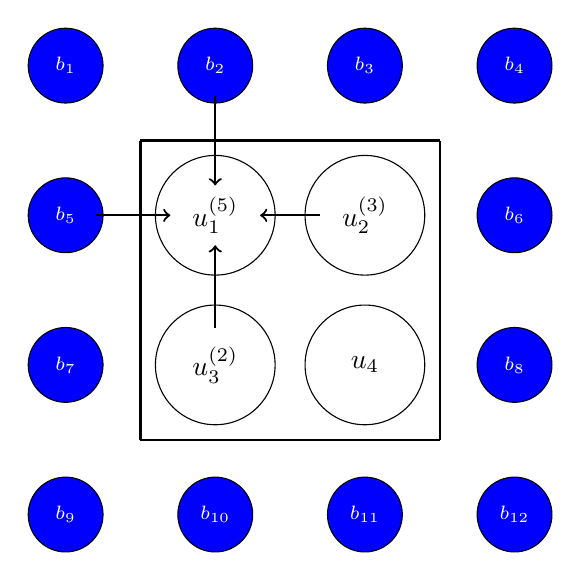
\begin{tikzpicture}[scale=1.9]
		% setup the nodes as small black circles
		\foreach \x in {0,...,3} {
			\foreach \y in {0,...,3} {
				\node[shape=circle,fill=black,scale=0.3] (\x-\y) at (\x,\y){}; 
				%labeling as \x-\y allows referencing inside of a foreach loop later
			}
		}
		
		% circle interior nodes with letters
		\foreach \mynode/\mytext in {1-2/$u_1^{(5)}$,2-2/$u_2^{(3)}$,1-1/$u_3^{(2)}$,2-1/$u_4$} {
			\draw[fill=white] (\mynode) circle (0.4cm) node {\mytext};
		}		
		
		% drawing interior/boundary box
		\draw[thick] (0.5,0.5) to (2.5,0.5); 
		\draw[thick] (0.5,0.5) to (0.5,2.5); 
		\draw[thick] (0.5,2.5) to (2.5,2.5); 
		\draw[thick] (2.5,2.5) to (2.5,0.5); 
		
		% label boundary nodes
		\foreach \mynode/\mytext in {0-3/$b_1$,1-3/$b_2$,2-3/$b_3$,3-3/$b_4$,
			0-2/$b_5$,0-1/$b_7$,3-1/$b_8$,3-2/$b_6$,
			0-0/$b_9$,1-0/$b_{10}$,2-0/$b_{11}$,3-0/$b_{12}$} {
			\draw[fill=blue,text=white] (\mynode) circle (0.25cm) node {{\scriptsize \mytext}};
		}	
		
		% drawing lines to show the nodes needed to update $u_1$
		\draw[->,thick] (0.2,2) to (0.7,2); 
		\draw[->,thick] (1,2.8) to (1,2.2); 
		\draw[->,thick] (1,1.25) to (1,1.8); 
		\draw[->,thick] (1.7,2) to (1.3,2); 
		\end{tikzpicture}
	\end{figure}
\end{frame}

\begin{frame}
	\frametitle{Classical approaches to parallelism}
	\begin{itemize}
		\item Synchronous Block Solvers:
			\begin{itemize}
				\item Each processor picks a block to update and uses the information from the prior iteration
					\begin{itemize}
						\item Think: 100 processors, 1000 blocks- processor 1 will update block 1, 101, 201, $\ldots$
					\end{itemize}
				\item Creates a synchronization point at the end of each iteration
			\end{itemize}
		\item Asynchronous Block Solvers:
			\begin{itemize}
				\item Each processor picks a block to update and uses the latest information available
					\begin{itemize}
						\item Data probably comes from a mix of iterations
					\end{itemize}
				\item No synchronization points, but less coordination
					\begin{itemize}
						\item Update ``levels'' can get out-of-sync; may need to assume a bound on how much
					\end{itemize}
				\item Convergence results tend to be asymptotic
			\end{itemize}
	\end{itemize}
\end{frame}

\begin{frame}
	\frametitle{Modern approaches to parallelism}
	\begin{itemize}
		\item Randomized Block Solvers:
			\begin{itemize}
				\item Each processor picks a block uniformly at random
				\item Can be synchronous or asynchronous
				\item Performance similar to asynchronous block solvers
			\end{itemize}
		\item Weighted Randomized Block Solvers:
			\begin{itemize}
				\item The probability distribution is weighted {\em before} calculation starts
					\begin{itemize}
						\item Ex: blocks with larger norm are favored, blocks with more non-zeros are favored
					\end{itemize}
			\end{itemize}
		\item Distributed Southwell:
			\begin{itemize}
				\item Non-randomized, asynchronous approach
				\item Each processor is assigned to a block and (independently) updates the equation with highest contribution to the residual of any coupled variable
			\end{itemize}
	\end{itemize}
\end{frame}

\begin{frame}
	\frametitle{``New'' approach}
	\begin{itemize}
		\item Make the random selection change dynamically 
		\item Goal is to gain some benefit of selecting the ``right'' blocks (similar to classical Southwell) without adding so much computational overhead that the total execution time is slower
		\item Based around monitoring which blocks contribute most to the residual $r = b - Ax$
		\item Periodically find and rank the component residuals (for the contribution of block $i$):
			\begin{equation}
				r_i = b_i - Ax_i
			\end{equation}
			and make the selection using a non-uniform distribution
	\end{itemize}
\end{frame}


\begin{frame}
	\frametitle{Residual data for finite-difference of 2D Laplacian}
	\begin{figure}[H]
		\centering
		\subfloat[Unsorted residuals]{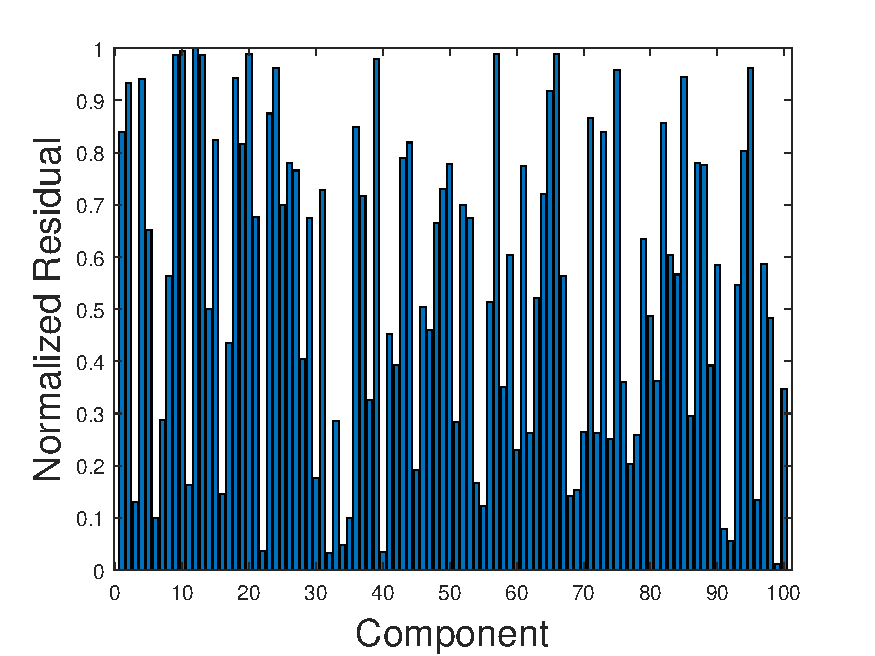
\includegraphics[width=0.45\textwidth]{images/init_resids_10x10.pdf}}
		\subfloat[Sorted residuals]{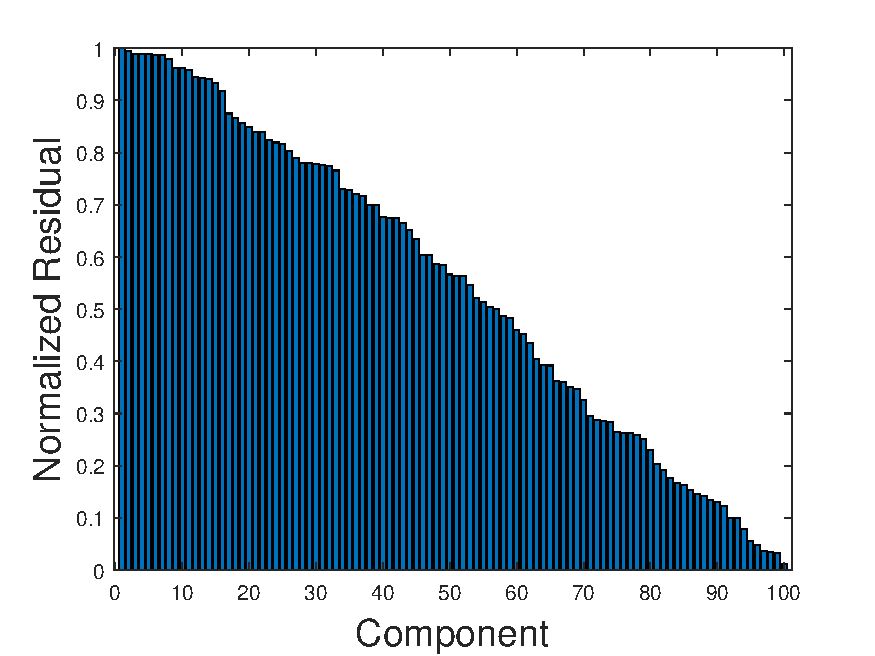
\includegraphics[width=0.45\textwidth]{images/init_resids_10x10_sorted.pdf}}
		\caption{Initial component residuals ($r_i / \max (r_i)$).}
		\label{fig:initial-residuals-laplacian}
	\end{figure}
\end{frame}

\begin{frame}
	\frametitle{Ranked residual data for finite-difference of 2D Laplacian}
	\begin{figure}[H]
		\centering
		\subfloat[Sorted Residuals, exponential distributions]{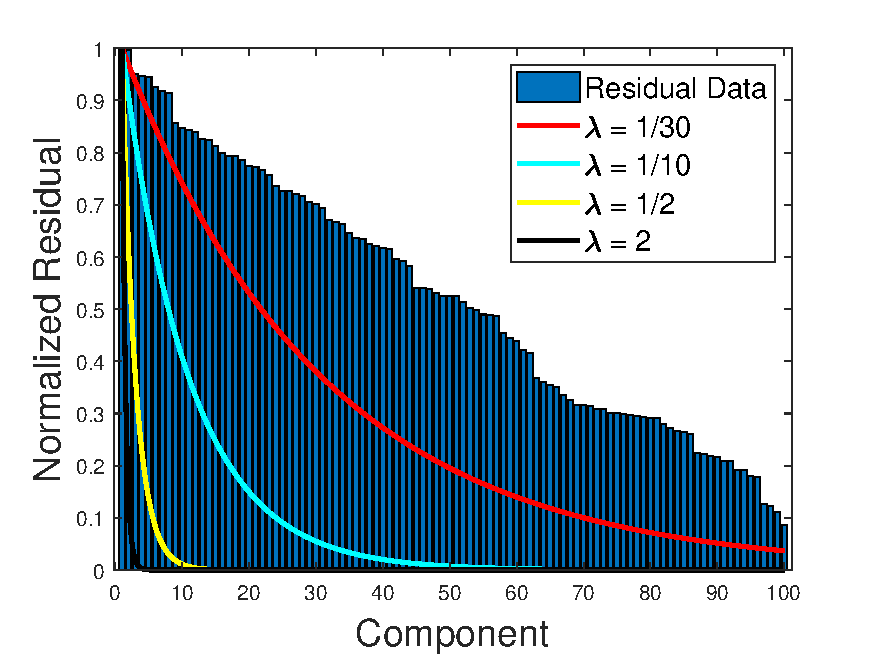
\includegraphics[width=0.45\textwidth]{images/exp_dist_overlay_10iter.pdf}}
		\subfloat[Sorted Residuals, triangular distributions]{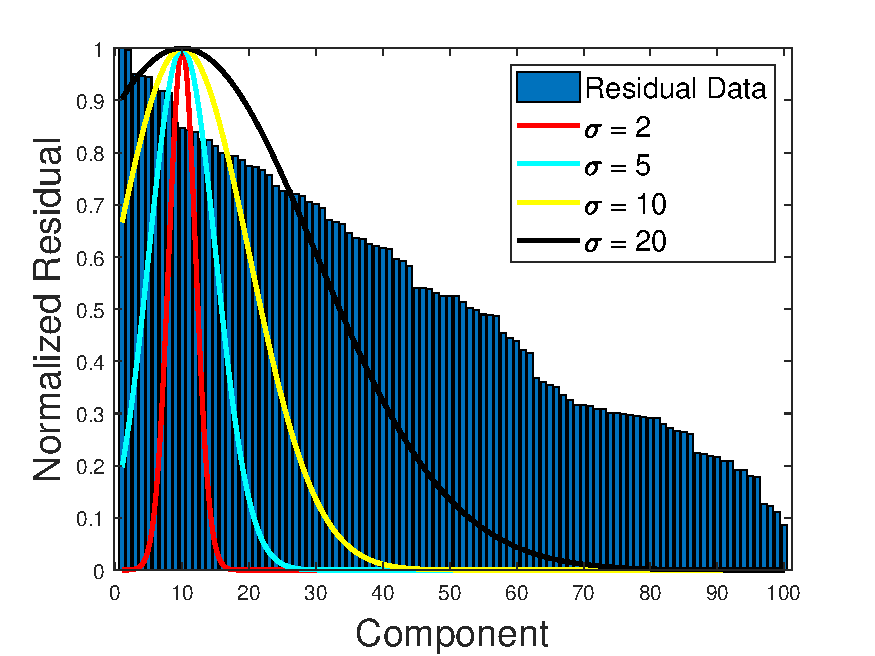
\includegraphics[width=0.45\textwidth]{images/normal_dist_overlay_10iter.pdf}}
	\end{figure}
	\begin{itemize}
		\item Need to balance computational cost associated with generating a ranked list and fitting a distribution with the benefit in doing so
	\end{itemize}
\end{frame}

\begin{frame}
	\frametitle{Solver data (Laplacian)}
	\begin{figure}[H]
		\centering
		\subfloat[2D problem (5-pt stencil, $10\times 10$ grid)]{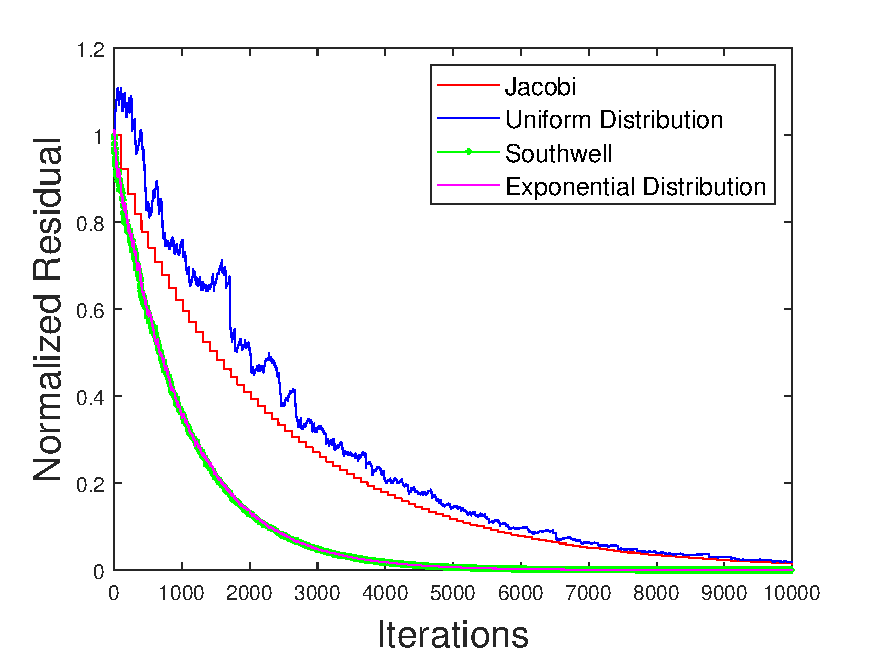
\includegraphics[width=0.45\textwidth]{images/res_10x10.pdf}}
		\subfloat[3D problem (27-pt stencil, $10 \times 10 \times 10$ grid)]{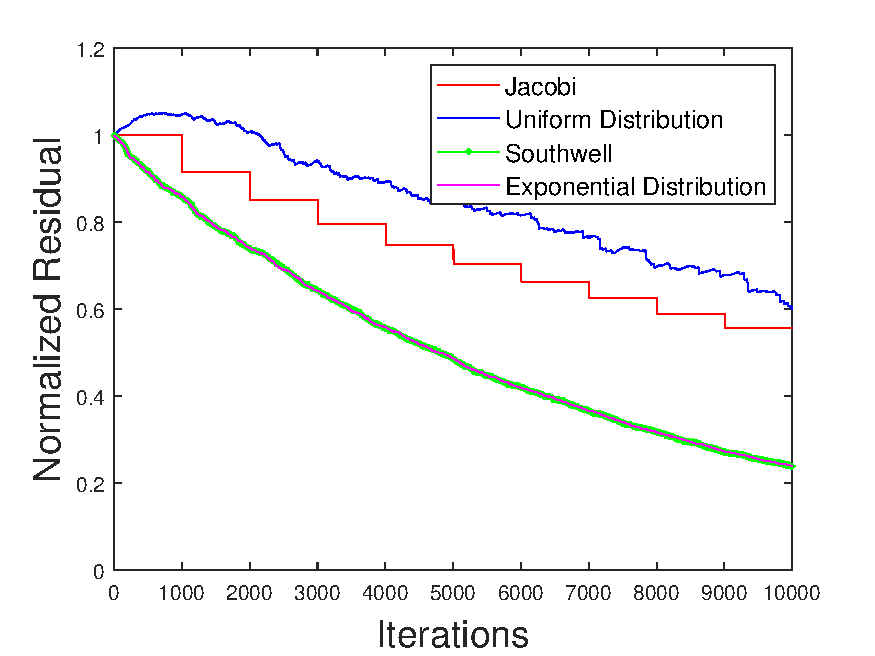
\includegraphics[width=0.45\textwidth]{images/res_3D_10x10x10.pdf}}
		\caption{Residual ($r / r_0$) progression for the first 10,000 iterations of four stationary methods solving the 2D (a) and 3D (b) Laplacian.}
	\end{figure}
\end{frame}

\begin{frame}
	\frametitle{Moving forward I}
	\begin{itemize}
		\item Viewing the iteration as a fixed point algorithm allows the use of successive differences:
				\begin{align}
					\delta^{(k+1)} &= \Vert x^{(k+1)} - x^{(k)} \Vert \\
					\delta^{(k+1)}_i &= \Vert x^{(k+1)}_i - x^{(k)}_i \Vert 
				\end{align}
			since termination occurs when $x^{(k+1)} \approx G \left( x^{(k)} \right)$, or when
				\begin{equation}
					\Vert x^{(k+1)} - x^{(k)} \Vert < \epsilon.
				\end{equation}
		\item Much less computationally expensive and exhibit similar behavior and trends
			\begin{itemize}
				\item Theory is significantly less developed
			\end{itemize}
	\end{itemize}
\end{frame}

\begin{frame}
	\frametitle{Moving forward II}
	\begin{itemize}
		\item Proving convergence as a per iteration reduction in the expected error
		\begin{itemize}
			\item Existing work proves relations such as (for synchronous, uniformly randomized, block Gauss-Seidel):
			\begin{equation}
			\mathbb{E}[\Vert x^{(k)} - x^* \Vert ] \leq \left( 1 - \frac{\beta (2 - \beta) \lambda_{min}}{n}\right)^k \Vert x^{(0)} - x^* \Vert^2_A
			\end{equation}
			\item General idea of proof: choose a (weighted) probability distribution so that the new distance from the solution is the old distance times some known quality (such as a residual)
		\end{itemize}
		\item Dealing with the distributed memory environment
			\begin{itemize}
				\item Most approaches to this problem analyze and experiment with shared memory environments (e.g. a single workstation/GPU)
				\item Extending to the distributed environment is non-trivial
			\end{itemize}
		\item Incorporating new solvers into more complex existing routines
	\end{itemize}
\end{frame}
 
\begin{frame}
	\frametitle{Moving forward III}
	\begin{itemize}
		\item Experimenting with different distributions (still chosen beforehand) and ranking methods and periodicities
		\item Dynamically fitting the residual or difference data with an evolving probability distribution
		\item Investigating the impact that different problems have
			\begin{itemize}
				\item If all blocks have equal contribution to the residual, using a non-uniform distribution has no benefit
				\item Are there problems that some approaches can handle that others can't?
			\end{itemize}
		\item Look into the performance inside of more complicated ``real world'' applications
			\begin{itemize}
				\item Do these small differences even matter?
			\end{itemize}
	\end{itemize}
\end{frame}

%\section{A (slightly more) formal approach}
%
%\begin{frame}
%	\frametitle{Notation (following Griebel and Oswald, 2012)}
%	\begin{itemize}
%		\item Let:
%			\begin{itemize}
%				\item $V$ be a separable Hilbert space
%				\item $a(\cdot, \cdot)$ be a continuous symmetric positive definite bilinear form on $V$
%				\item $F$ be a bounded linear functional on $V$
%				\item $V_a$ represent the Hilbert space with scalar product given by the bilinear form $a(\cdot, \cdot)$ 
%			\end{itemize}
%		\item The problem becomes a variational problem, (iteratively) find $u \in V$ such that
%			\begin{equation}
%				a(u,v) = F(v) 
%			\end{equation}
%			 for all $v \in V$
%	\end{itemize}
%\end{frame}
%
%\begin{frame}
%	\frametitle{Notation (continued)}
%	\begin{itemize}
%		\item The iteration from before becomes an iterative subspace correction scheme
%		\item Let $V_a$ be represented by a finite collection of Hilbert spaces, $V_{a_i}$, along with inner products $a_i(\cdot, \cdot)$, and bounded linear operators, $R_i: V_{a_i} \rightarrow V_a$ as follows:
%			\begin{equation}
%				V_a = \sum_{i=1}^N R_i V_{a_i} = \lbrace v = \sum_{i=1}^N R_i v_i : v_i \in V_{a_i}, i = 1, \ldots, N \rbrace
%			\end{equation}
%		\item As before, the subspaces don't have to be disjoint but they can be thought of that way
%	\end{itemize}
%\end{frame}
%
%\begin{frame}
%	\frametitle{...and further}
%	\begin{itemize}
%		\item There are upper bounds on the $R_i$ operators
%			\begin{equation}
%				a(R_i v_i, R_i v_i) \leq \gamma_i a_i (v_i, v_i)
%			\end{equation}
%		\item Define operators $T_i: V_a \rightarrow V_{a_i}$
%			\begin{equation}
%				a_i(T_i v, v_i) = a(v, R_i v_i)
%			\end{equation}
%		\item Define the error at each iteration (in order to compute a residual) as
%			\begin{equation}
%				e^{(k)} = u - u^{(k)}
%			\end{equation}
%			which can be solved since the variational problem at each iteration can be solved without knowledge of $u$
%	\end{itemize}
%\end{frame}
%
%\begin{frame}
%	\frametitle{Bringing it back}
%	\begin{itemize}
%		\item In terms of the block methods discussed earlier for solving $Ax = b$, where $A$ is SPD:
%			\begin{itemize}
%				\item $V = \mathbb{R}^n$
%				\item The space splitting is based on the coordinate vectors, $e_i$ (so each $V_{a_i}$ is a copy of $\mathbb{R}$)
%				\item $a(x,y) = y^T Ax$, $F(x) = b^T x$, and $a_i(x_i, y_i) = x_i y_i$
%				\item The operators $R_i$ go from $V_{a_i}$ to $V_a$ and can be defined by $R_i(x_i) = x_i e_i$
%				\item The bounds $\gamma_i$ are just there to ensure the iterate mapping is ``contractive''; setting them to the diagonal elements $a_{ii}$ is sufficient
%				\item The operators $T_i$ are defined by the variational problem (which is controlled by $a_i(\cdot,\cdot)$ and $a(\cdot,\cdot)$); here $T_i v = (Av)_i$
%			\end{itemize}
%	\end{itemize}
%\end{frame}
%
%\begin{frame}
%	\frametitle{General algorithm}
%	\begin{algorithm}[H]
%		\DontPrintSemicolon
%		\KwIn{Space splitting-$V_a$, operators $R_i, T_i$, initial guess $u^{(0)} \in V_a$, relaxation parameter $\beta$, bounds $\gamma_i$}
%		\For {$k = 1, 2, \ldots$ until convergence} {
%			Compute the residuals, $r_i^{(k)} = T_i e^{(k)}$ \;
%			Choose an index, $i^*$, associated with a desired subspace \;
%			Set $u^{(k)} = u^{(k-1)} + \frac{\beta}{\gamma_i} R_{i^*} r_{i^*}^{(k-1)}$ \;
%		}
%	\end{algorithm}
%\end{frame}

\section{Related areas}

\begin{frame}
	\frametitle{Related areas}
	\begin{itemize}
		\item While linear solvers are prevalent throughout science and engineering, the idea of using weighted randomization could find uses in other key areas
		\item Example: convex optimization 
			\begin{itemize}
				\item stochastic gradient descent, and variants thereof
				\item current research mainly focuses on uniformly selecting components, but some studies have examined using a Southwell-like approach with some success
					\begin{itemize}
						\item using weighted randomization may allow a blend between the two approaches
					\end{itemize}
			\end{itemize}
	\end{itemize}
\end{frame}










\end{document}